\documentclass{article}
\usepackage[utf8]{inputenc}
\usepackage{amsmath}
\usepackage{amsfonts}
\usepackage{graphicx}

\title{Written Assignment Unit 4\\
Math 1201- College Algebra.
}
\author{Instructor - Casmir Onyeneke}
\date{September 2021}


\begin{document}

\maketitle

\section*{Question 1}
\title\textbf{Composite Functions}\\
Question Statement: What can be said about the domain of the function \textit f o g where ${\textit{f(y)} = \frac{4}{y-2}}$ and ${\textit{g(x)} = \frac{5}{3x-1}}$ ? Express in terms of a union of real numbers.\\
\textbf{Solution}
$${\textit{f(y)} = \frac{4}{y-2}}$$
$${\textit{g(x)} = \frac{5}{3x-1}}$$
\\The composite function \textit{f o g} can be expressed as

$${\textit{f o g} = \textit{f(g(x))}}$$
$${\textit{f o g} = \textit f\left(\frac{5}{3x-1}\right)}$$
$${\textit{f o g} = \frac{4}{\frac{5}{3x-1}-2}}$$
$${\textit{f o g} = \frac{4(3x-1)}{5 - (6x - 2)}}$$
$${\textit{f o g} = \frac{12x-4}{5 + 2 - 6x}}$$
$${\textit{f o g} = \frac{12x-4}{7 - 6x}}$$

The Domain of this composite function is:
$${7 - 6x \neq 0}$$
$${6x \neq 7}$$
$${x \neq \frac{7}{6}}$$
So therefore the domain expressed in interval notation is\\
$${(-\infty, \frac{7}{6})\cup(\frac{7}{6}, \infty)}$$ 
\\Below is the graph of \textit{f, g and f o g }\\
\\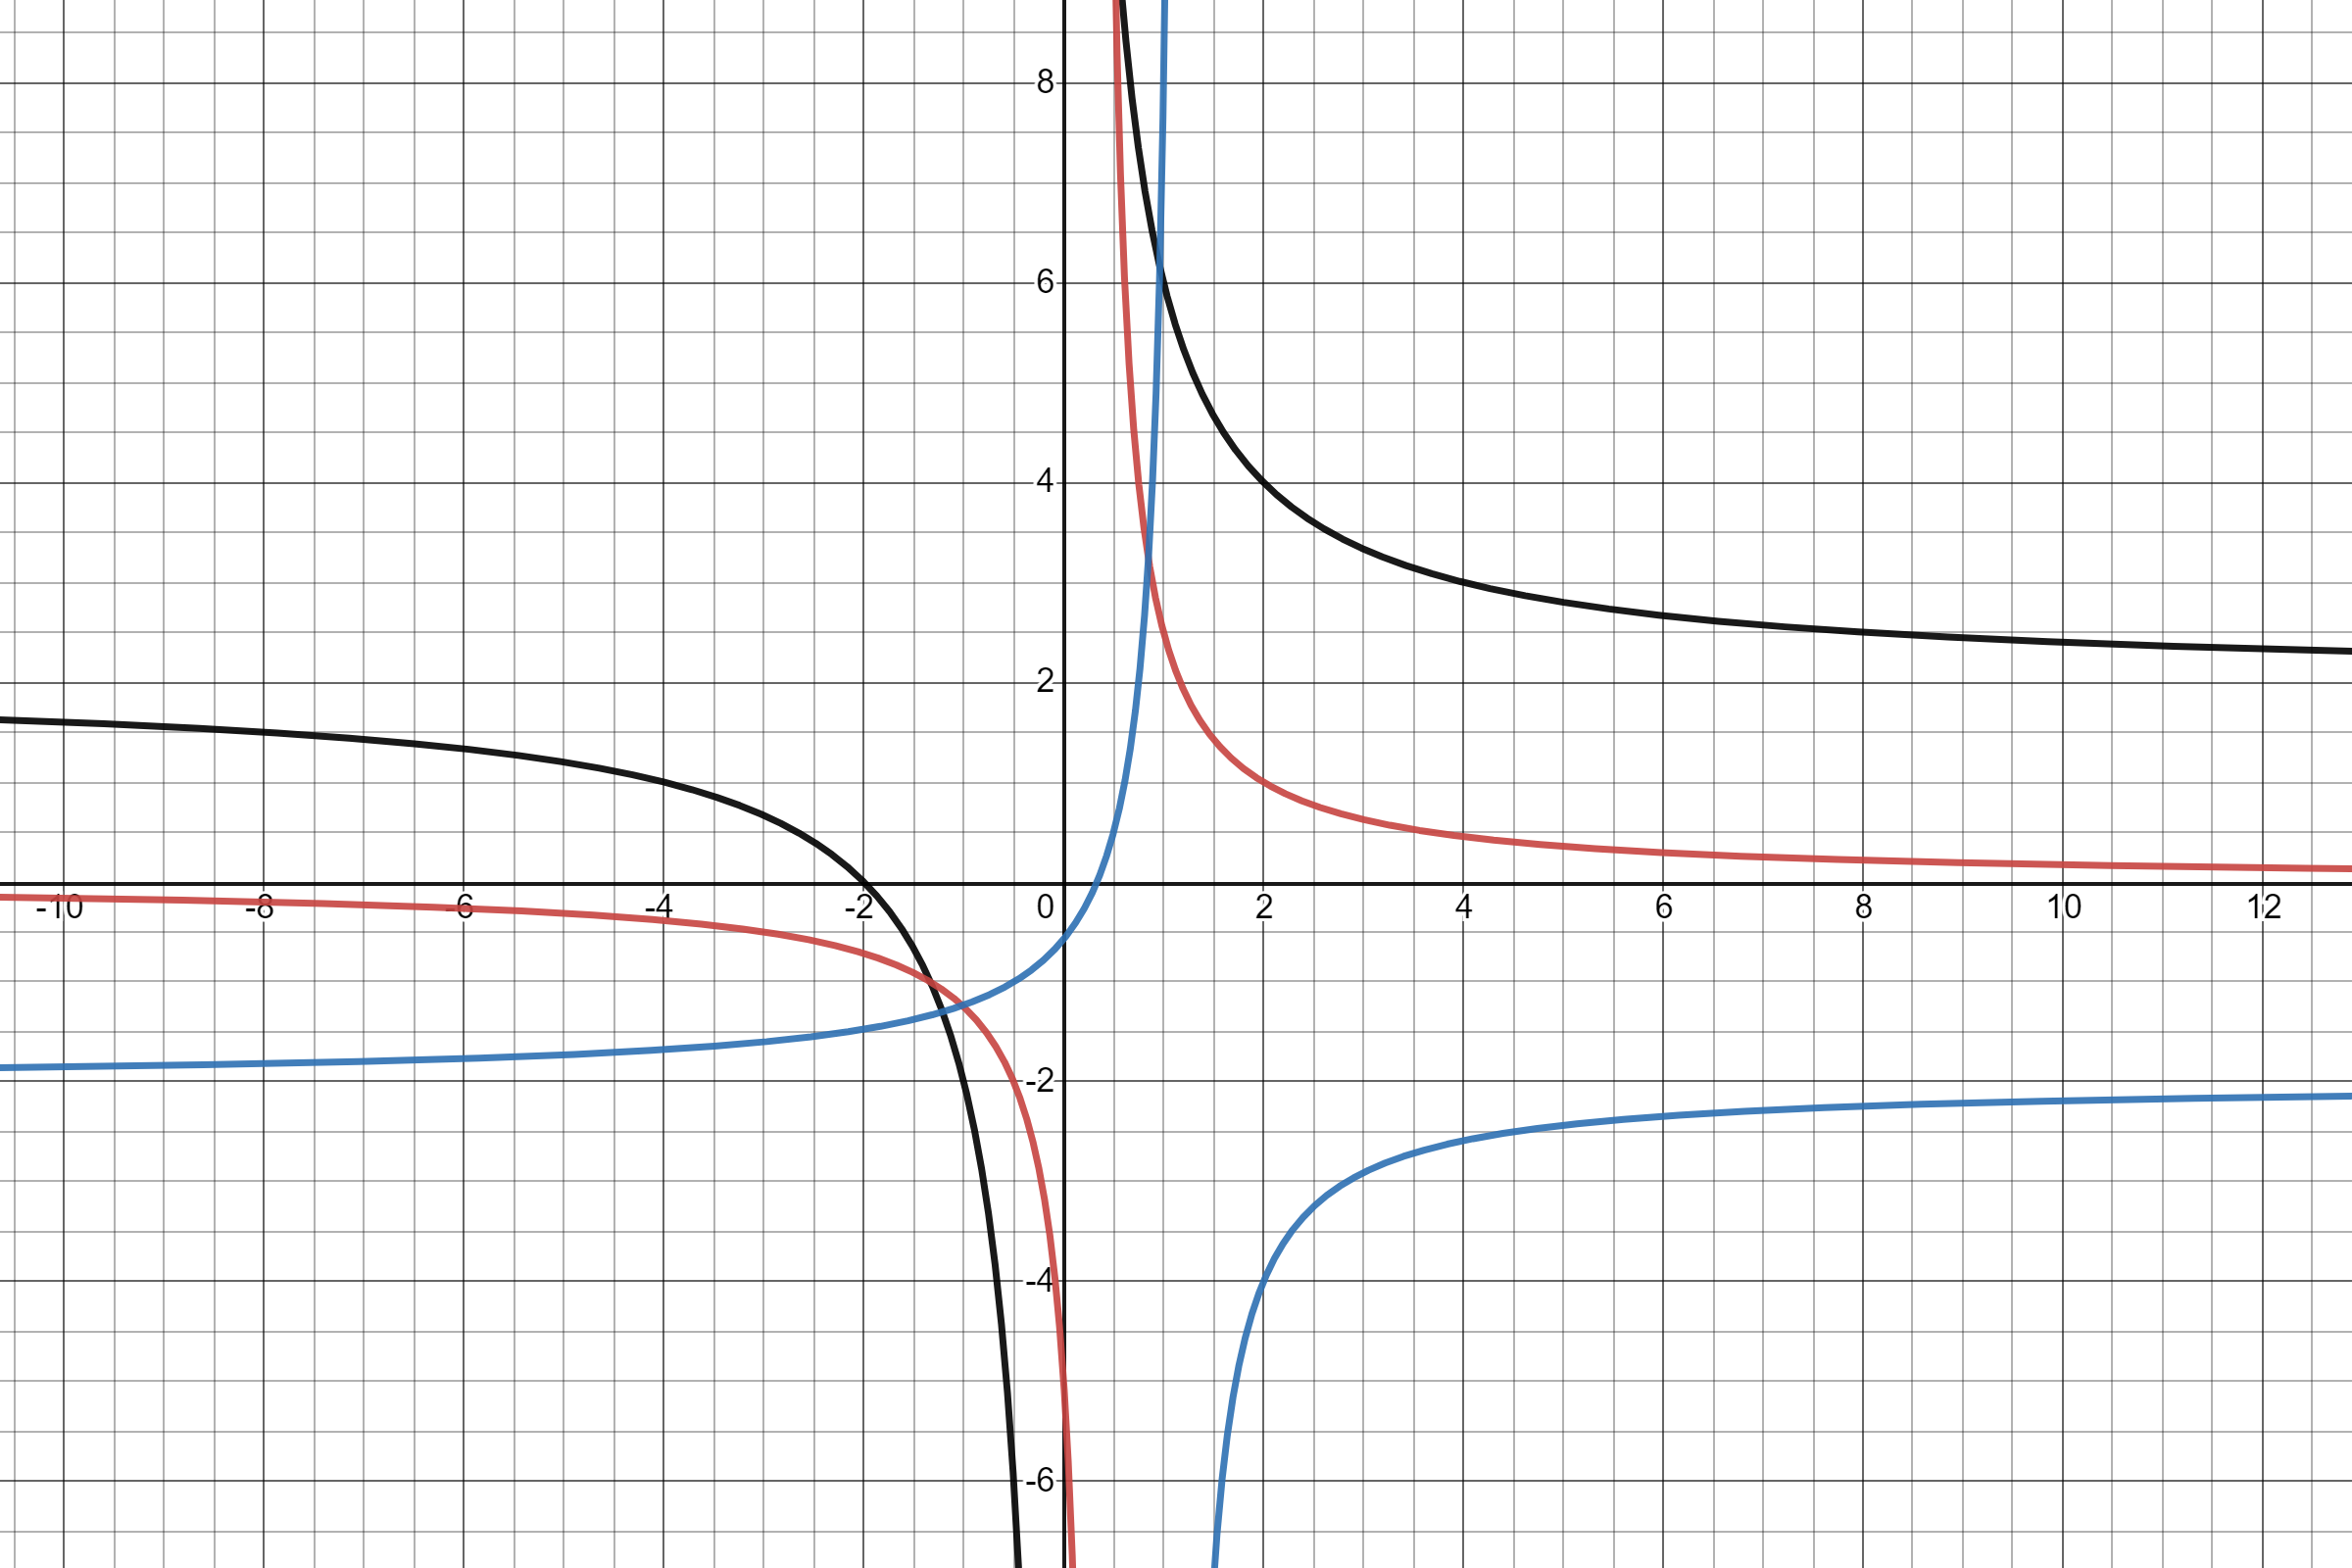
\includegraphics[scale = 0.15]{wAQ1}\\
\\${\textit{f(y)} = \frac{4}{y-2}}$ is the black curve
\\${\textit{g(x)} = \frac{5}{3x-1}}$ is the red curve
\\${\textit{f o g} = \frac{12x-4}{7 - 6x}}$ is the blue curve\\




\section*{Question 2}
\title\textbf{Inverse Functions}
\\Question Statement: Find the inverse of the function ${\textit{f(x)}=4+\sqrt{x-2}}$
\\state the domains and ranges of both the function and the inverse function in terms of intervals of real numbers.
\\\textbf{Solution}
$${\textit{f(x)}=4+\sqrt{x-2}}$$
We can say that ${\textit{f(x)} = y}$
$${y = 4+\sqrt{x-2}}$$
Making ${x}$ the subject of the equation 
$${y = 4+\sqrt{x-2}}$$
subtract 4 from both the LHS and RHS
$${y - 4 = \sqrt{x-2}}$$
$${\sqrt{x-2} = y - 4 }$$
Square both the LHS and RHS
$${(\sqrt{x-2})^2 = (y - 4)^2 }$$
$${x - 2 = (y - 4)^2 }$$
Add 2 to both the LHS and RHS
$${x = (y - 4)^2 + 2}$$
$${y = x^2 - 8x + 16 + 2 }$$
$${y = x^2 - 8x + 18 }$$
\\Therefore the inverse function of ${\textit{f(x)}=4+\sqrt{x-2}}$  is  
${\textit f^{-1}(x) = (x - 4)^2 + 2 }$
$${\textit f^{-1}(x) = x^2 - 8x + 18 }$$



\section*{Question 3}
\title{Question 2 Contd.}
\\Question Statement: Using the function from Q2, go to www.desmos.com/calculator and obtain the graph of \textit{f}, its inverse and, ${g(x) = x}$ in the same system of axes. About what pair (a,a) are (11, 7) and (7, 11) reflected about?
\\\textbf{Solution}\\
The Domain of ${\textit{f(x)}=4+\sqrt{x-2}}$ is 
$${x - 2 \geq 0}$$
$${x \geq 2}$$
Therefore the domain is $${[2, \infty)}$$
The range of ${\textit{f(x)}=4+\sqrt{x-2}}$ is $${[4,\infty)}$$ for ${x=2}$\\
\\\title{Inverse Function}\\
For the inverse of the function, sincethe domain of the inverse function is range of the original function and the range of the inverse function is the domain of the original function(Abramson, 2017).
\\The domain of the inverse function is therefore given as $${[4,\infty)}$$
And the range is $${[2,\infty)}$$
\\The graph of the following functions is shown below\\
$${\textit{f(x)} = 4+\sqrt{x-2}\quad \text{is the purple curve}}$$ 
$${\textit f^{-1}(x) = (x - 4)^2 + 2 \quad \text{is the black curve}}$$
$${g(x)=x\quad \text{is the red straight line}}$$
\\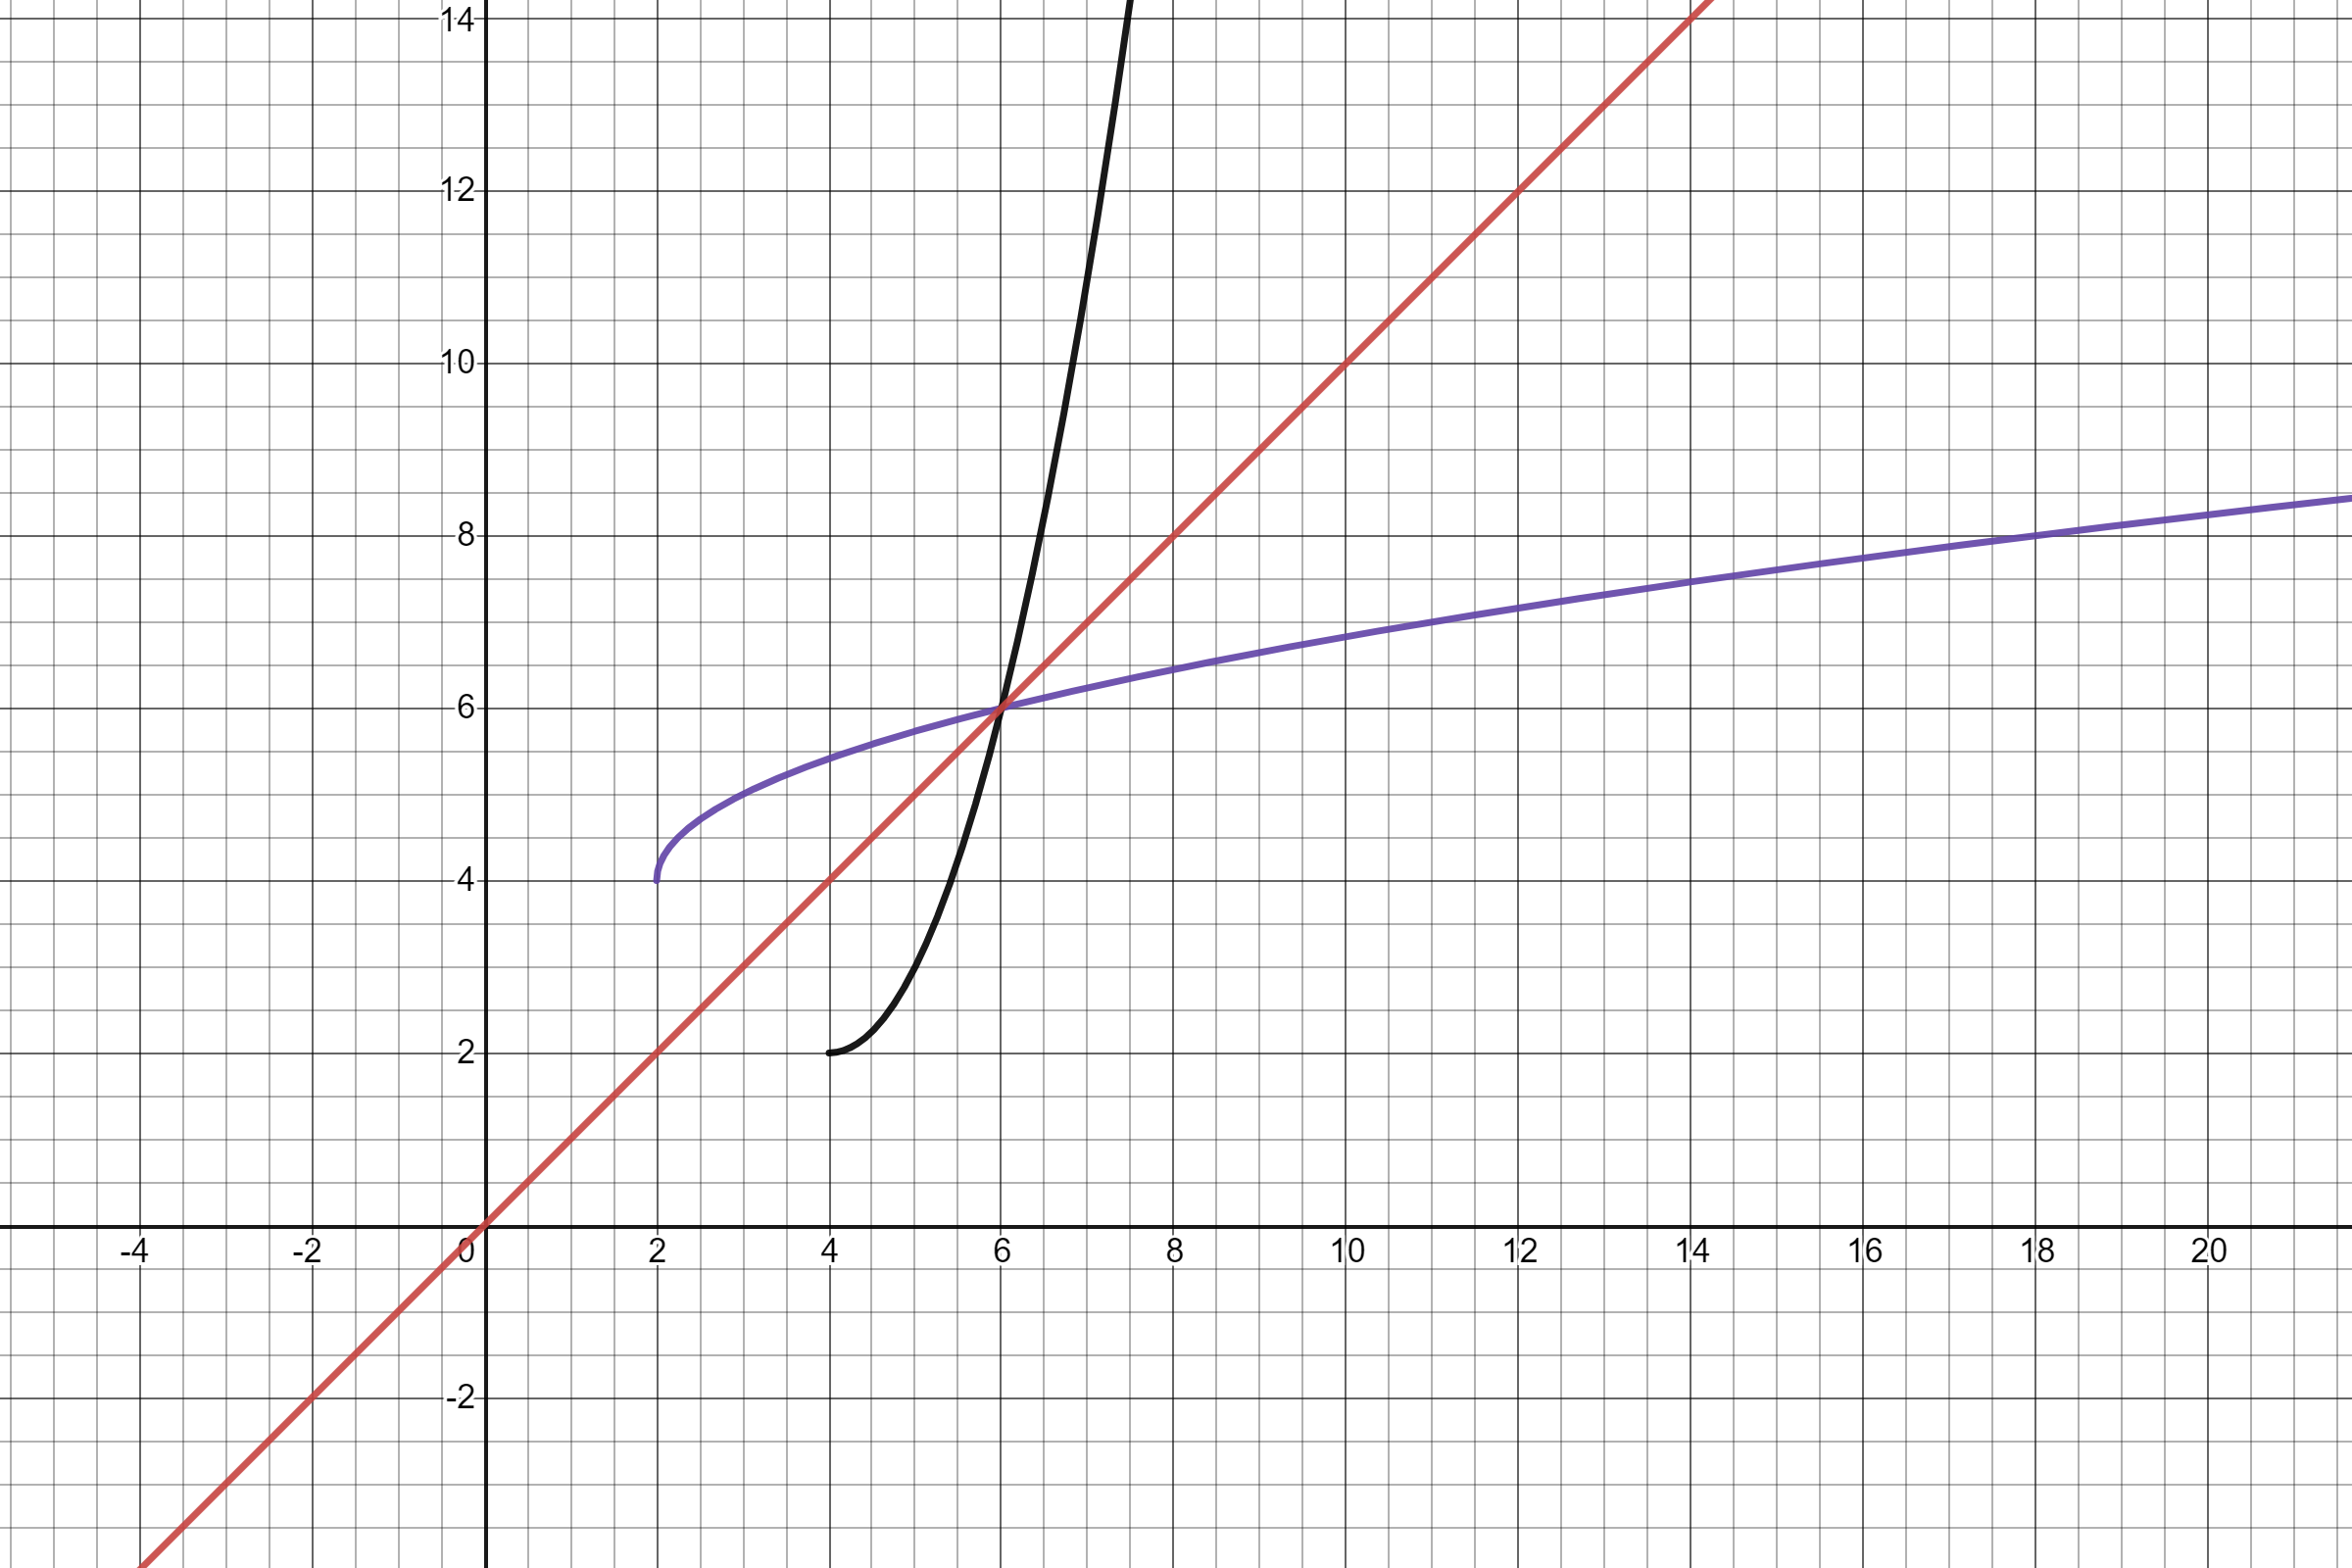
\includegraphics[scale = 0.15]{waQ3}\\
\\Finding the slope of the points (7,11) and (11,7)
$${m=\frac{7-11}{11-7}}$$
$${m=\frac{-4}{4}}$$
$${m=-1}$$

using the slope-intercept form (7, 11)
$${y = mx + b}$$
$${11 = -1(7) + b}$$
$${11 = -7 + b}$$
$${b = 18}$$
$${y = -x + 18}$$
\\The graph is shown below.\\
\\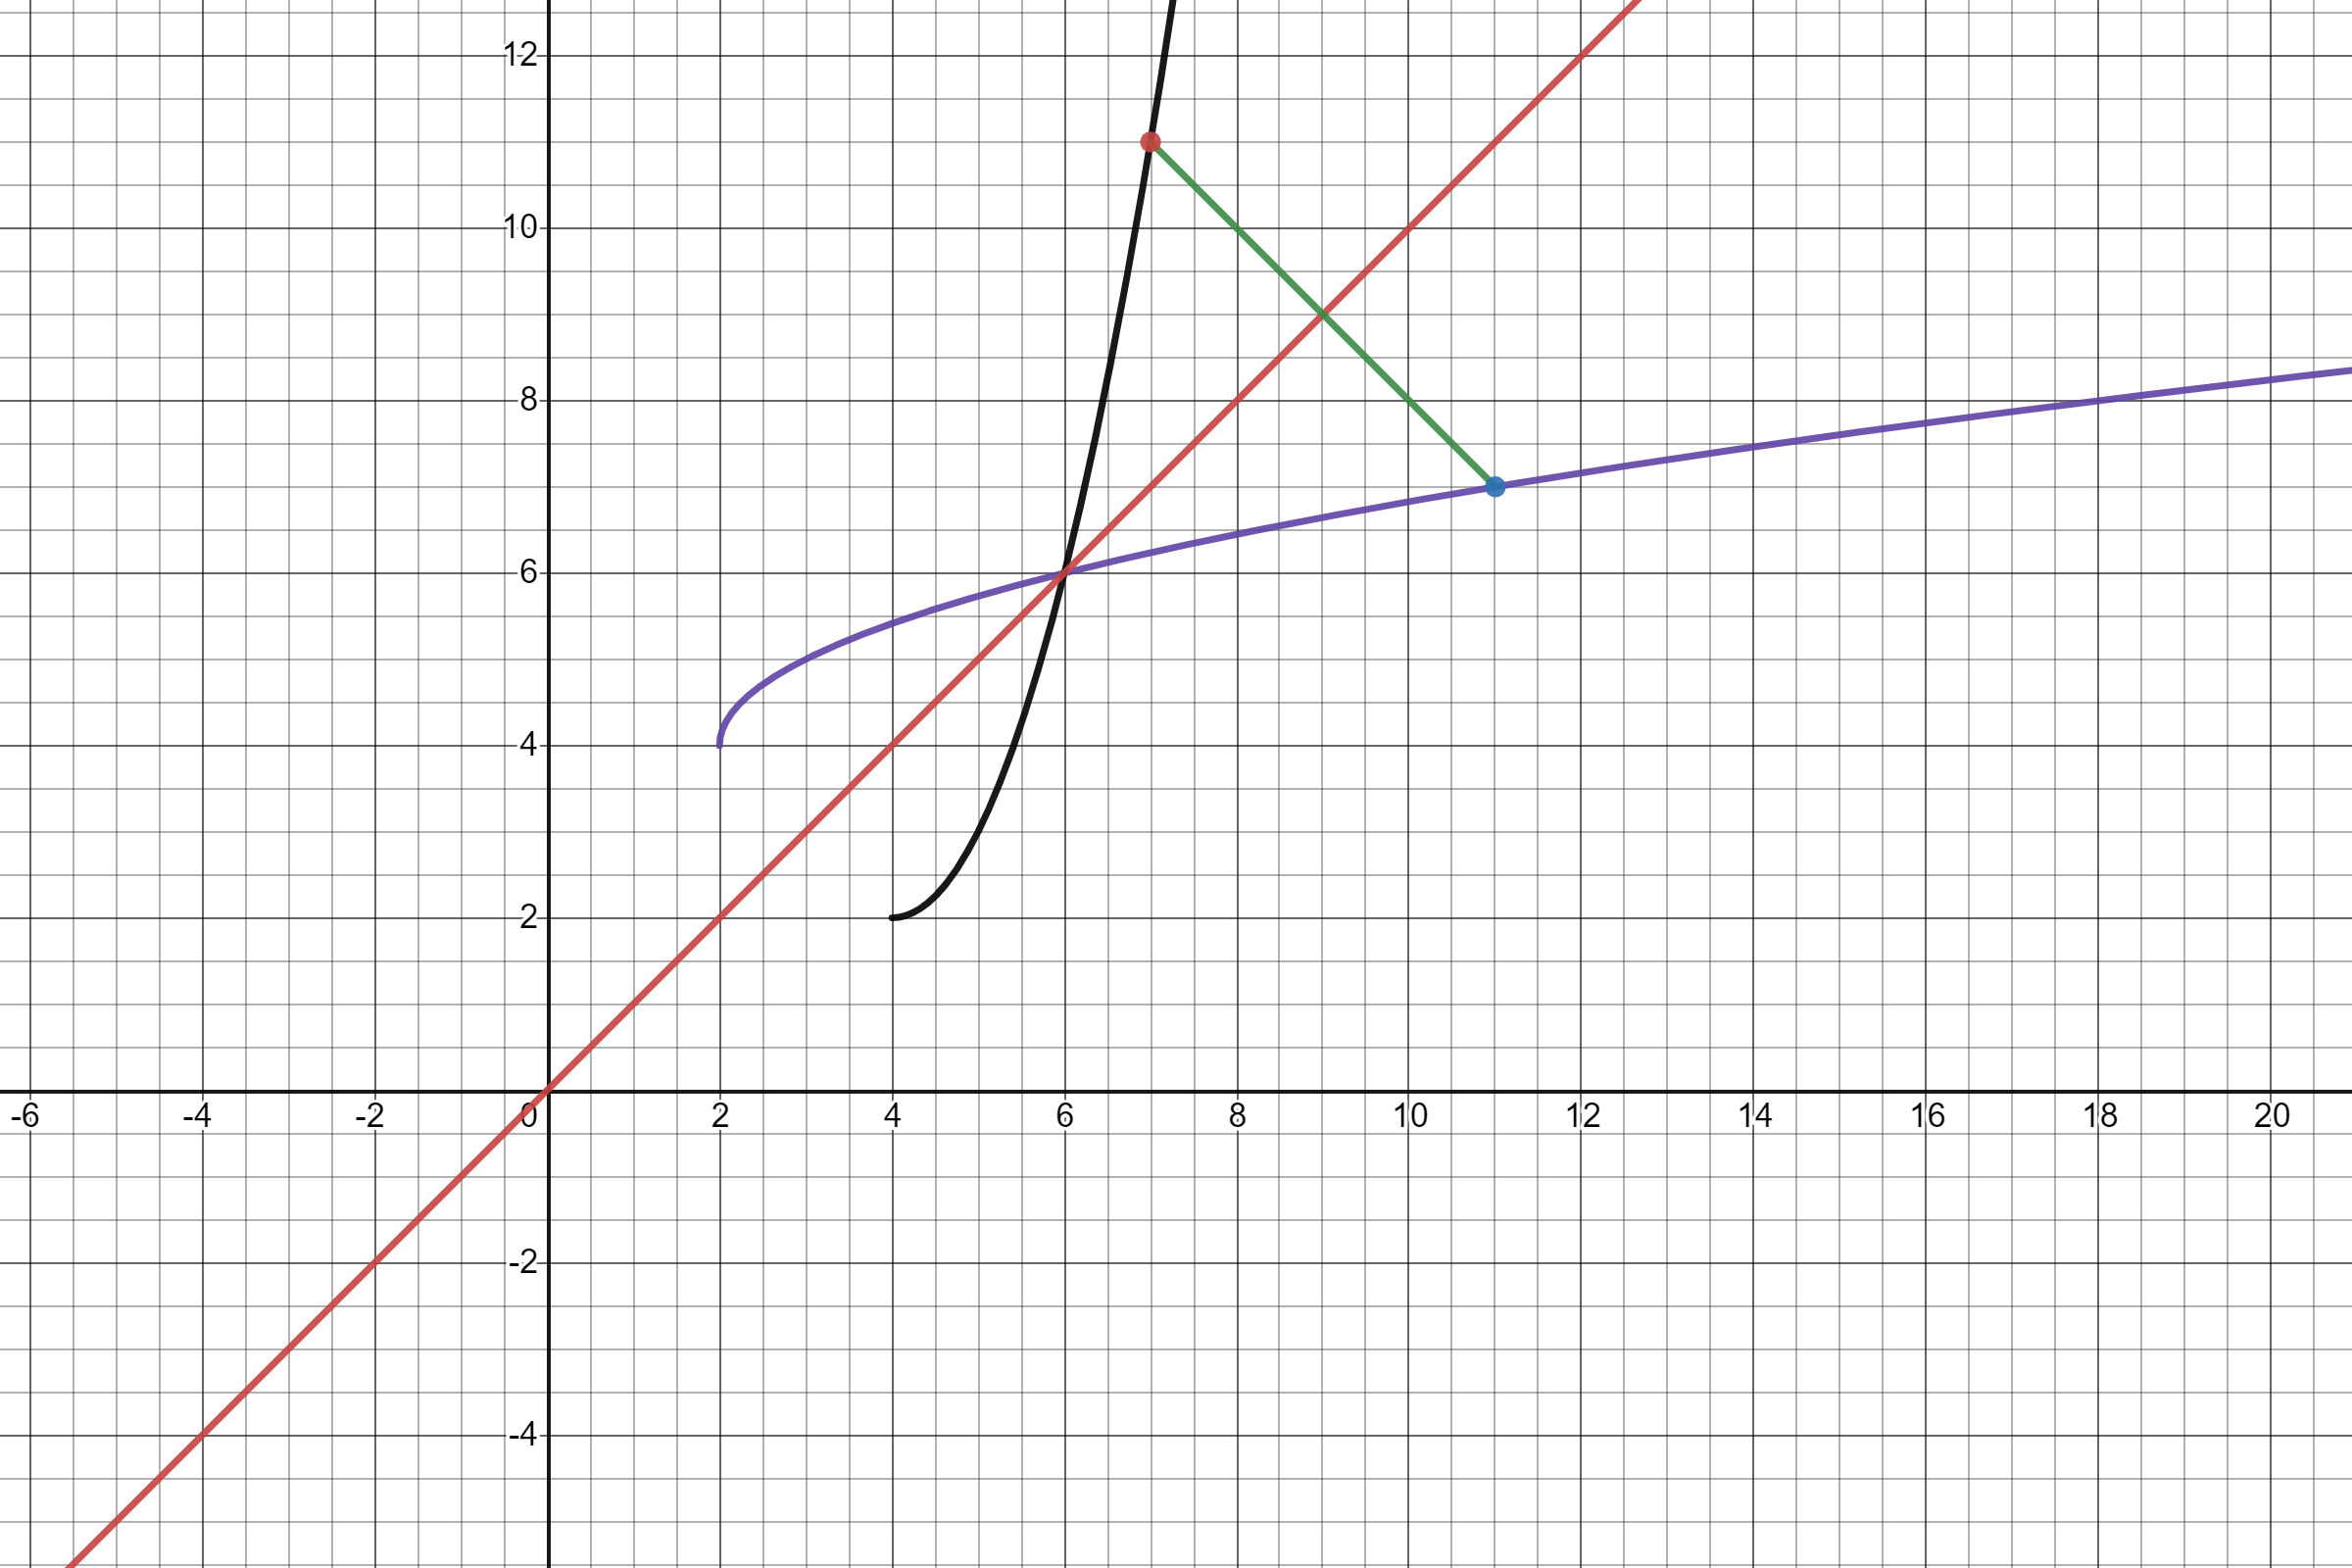
\includegraphics[scale = 0.15]{wa4Q3}\\
\\from the graph the point (7,11) and (11,7) are reflected about the point (9,9).

\section*{REFERENCES}
Abramson, J. (2017). \textit{Algebra and trigonometry}. OpenStax, TX: Rice University. Retrieved
from https://openstax.org/details/books/algebra-and-trigonometry
\end{document}